\section{Файловые диалоги и работа с файлами}
\verb|Задание.| Создать таблицу Student. В другой файл вывести студентов, у которых сдана сессия. (Вариант 1)

Для выполнения данного задания была разработна форма, содержащая два элемента 
\verb|DataGridView|, шесть элементов \verb|Button|, элементы \verb|OpenFileDialog| и \verb|SaveFileDialog| для 
работы с файлами, и элемент \verb|ErrorProvider| (см. рисунок \ref{fig:files_const}).

\begin{figure}[H]
\centering
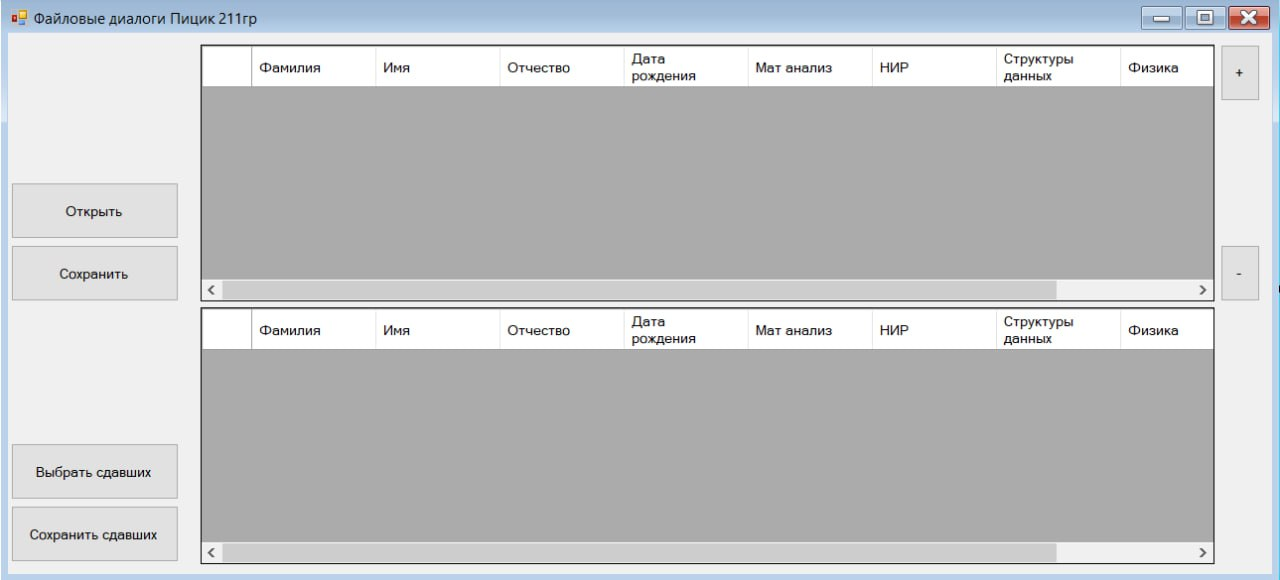
\includegraphics[scale=.45]{../img/files/files_konstructor.jpg}
\caption{Итоговый вид окна}
\label{fig:files_const}
\end{figure}

У элементов формы изменены значения некоторых свойств. С полным списком 
измененных свойств можно ознакомиться в таблице \ref{tab:files}.

\begin{table}[H]
    \small
    \caption{Значение атрибутов элементов формы}
    \begin{tabular}{|l|l|}\hline
        \multicolumn{2}{|l|}{Форма}\cr\hline
        \verb"Text" & Файловые диалоги Пицик 211гр.\cr\hline
        \multicolumn{2}{|l|}{DataGridView для ввода}\cr\hline
        \verb"(Name)" & data\_inuput\cr\hline
        \verb"AllowUserToAddRows" & False\cr\hline
        \verb"AllowUserToDeleteRows" & False\cr\hline
        \multicolumn{2}{|l|}{DataGridView для вывода}\cr\hline
        \verb"(Name)" & data\_output \cr\hline
        \verb"AllowUserToAddRows" & False\cr\hline
        \verb"AllowUserToDeleteRows" & False\cr\hline
        \multicolumn{2}{|l|}{Кнопка <<Открыть>>}\cr\hline
        \verb"(Name)" & btn\_open \cr\hline
        \verb"Text" & Открыть \cr\hline
        \multicolumn{2}{|l|}{Кнопка <<Сохранить>>}\cr\hline
        \verb"(Name)" & btn\_save \cr\hline
        \verb"Text" & Сохранить \cr\hline
        \multicolumn{2}{|l|}{Кнопка <<Выбрать сдавших>>}\cr\hline
        \verb"(Name)" & btn\_choose \cr\hline
        \verb"Text" & Выбрать сдавших \cr\hline
        \multicolumn{2}{|l|}{Кнопка <<Сохранить сдавших>>}\cr\hline
        \verb"(Name)" & btn\_savechoose \cr\hline
        \verb"Text" & Сохранить сдавших\cr\hline
        \multicolumn{2}{|l|}{Кнопка <<+>>}\cr\hline
        \verb"(Name)" & btn\_add \cr\hline
        \verb"Text" & + \cr\hline
        \multicolumn{2}{|l|}{Кнопка << - >>}\cr\hline
        \verb"(Name)" & btn\_remove \cr\hline
        \verb"Text" & - \cr\hline
        \multicolumn{2}{|l|}{Файловые диалог <<Открыть>>}\cr\hline
        \verb"(Name)" & open\_fd \cr\hline
        \verb"Title" & Открыть файл \cr\hline
        \verb"Filter" & Текстовые файлы (*.txt) | *.txt | Все файлы (*.*) | *.*\cr\hline
        \multicolumn{2}{|l|}{Файловые диалог <<Сохранить>>}\cr\hline
        \verb"(Name)" & save\_fd \cr\hline
        \verb"Title" & Сохранить файл \cr\hline
        \verb"Filter" & Текстовые файлы (*.txt) | *.txt | Все файлы (*.*) | *.*\cr\hline
    \end{tabular}
    \label{tab:files}
\end{table}

При нажатии кнопки <<Открыть>> открывается окно, позволяющее выбрать файлы форматов, заданных 
в свойстве \verb|Filter| для элемента \verb|OpenFileDialog| (см. рисунок \ref{fig:files_open}) \cite{book_beginners}.

\begin{figure}[H]
\centering
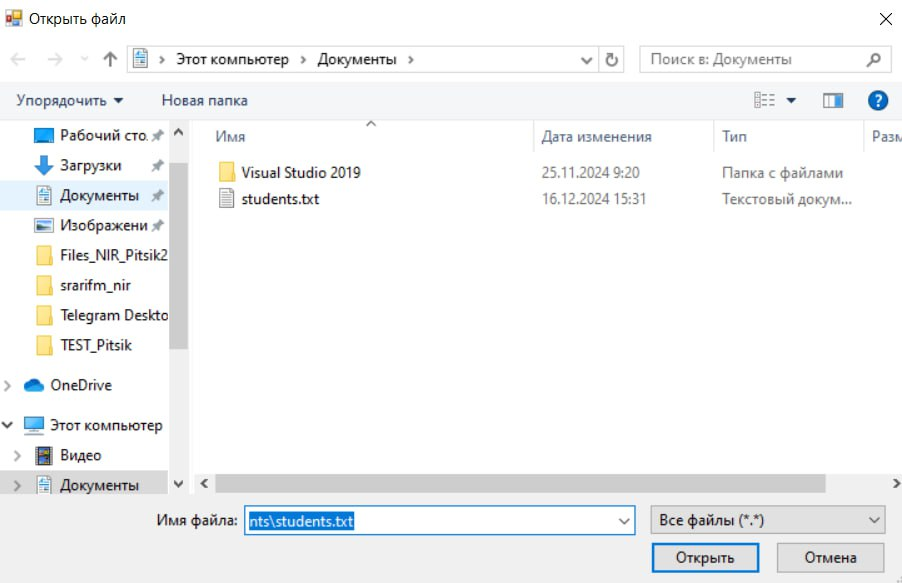
\includegraphics[scale=.65]{../img/files/files_open.jpg}
\caption{Открытие файла}
\label{fig:files_open}
\end{figure}

Для кнопнки <<Открыть>> был разработан следующий код:
\begin{minted}[linenos, breaklines=true, style=bw, fontsize=\small]{cpp}
private: System::Void btn_open_Click(System::Object^ sender, System::EventArgs^ e) {
    error_prov->Clear();

//открываем поток 
    System::IO::Stream^ myStream;
    if (this->openFileDialog->ShowDialog() == System::Windows::Forms::DialogResult::OK)
  //если успешно найден файл
      if ((myStream = openFileDialog->OpenFile()) != nullptr)
      {
//задаем кодировку чтения
        System::IO::StreamReader^ sr = gcnew System::IO::StreamReader(
          myStream, System::Text::Encoding::GetEncoding(1251)
        );
//заполняем dgv
        int row = 0;
        System::String^ str1 = "";
        while (sr->Peek() > -1)
        {
          str1 = sr->ReadLine();
          array<String^>^ words = str1->Split(' ');
          dgv_input->Rows->Add(words);
        }
//закрываем поток
        sr->Close();
      }
  }
\end{minted}

В случае сохранения файла, необходимо нажать кнопку <<Сохранить>>, фрагмент кода которой представлен ниже \cite{book_gui}.
\begin{minted}[linenos, breaklines=true, fontsize=\small, style=bw]{cpp}
System::IO::Stream^ myStream;
//открываем окно сохранения файла
      if (this->saveFileDialog->ShowDialog() == System::Windows::Forms::DialogResult::OK)
      {
        if ((myStream = saveFileDialog->OpenFile()) != nullptr)
        {
//запись файла
          System::IO::StreamWriter^ sw = gcnew System::IO::StreamWriter(myStream, System::Text::Encoding::GetEncoding(1251));
//считываем с итоговой таблицы
          for (int i = 0; i < dgv_output->RowCount; ++i)
          {
            String^ s;
            for (int j = 0; j < dgv_output->ColumnCount; ++j)
              s += System::Convert::ToString(dgv_output->Rows[i]->Cells[j]->Value) + " ";
//записываем строку
            sw->WriteLine(s);
          }
//закрываем поток
          sw->Close();
        }
      }
\end{minted}

С остальными кодами можно ознакомиться в приложении \ref{app:codes}.

При запуске программы открывается окно (см. рисунок \ref{fig:files_res}).
\begin{figure}[H]
\centering
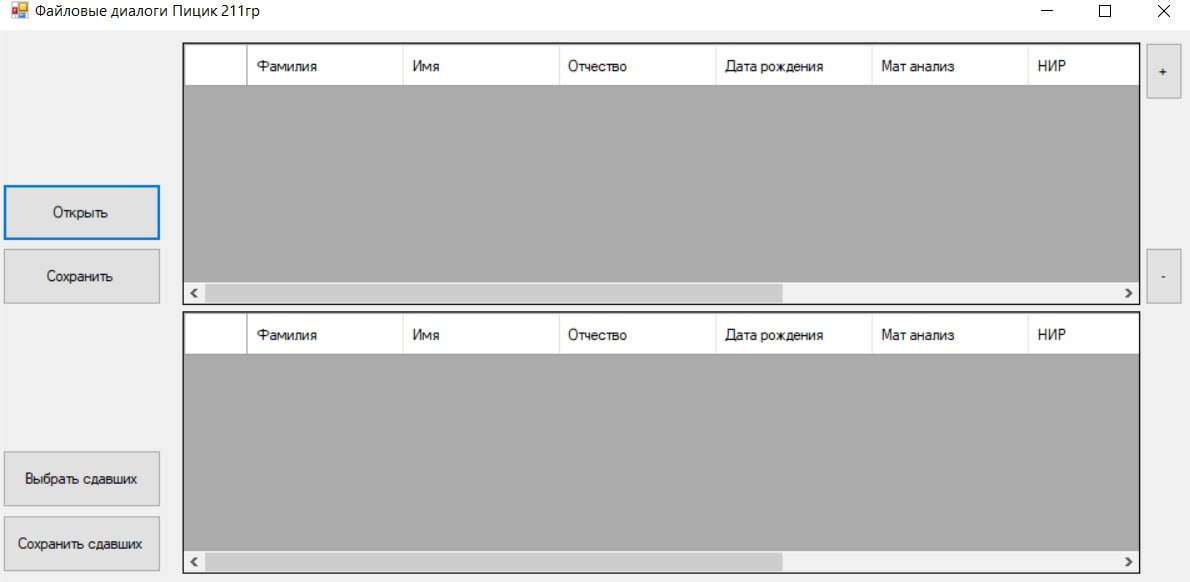
\includegraphics[scale=.45]{../img/files/files_res.jpg}
\caption{Окно приложения <<Файловые диалоги>>: запуск программы}
\label{fig:files_res}
\end{figure}

При нажатии на кнопку <<Выбрать сдавших>> в нижний элемент \verb|DataGridView| выводится список 
сдавших студентов (см. рисунок \ref{fig:files_choose}).
\begin{figure}[H]
\centering
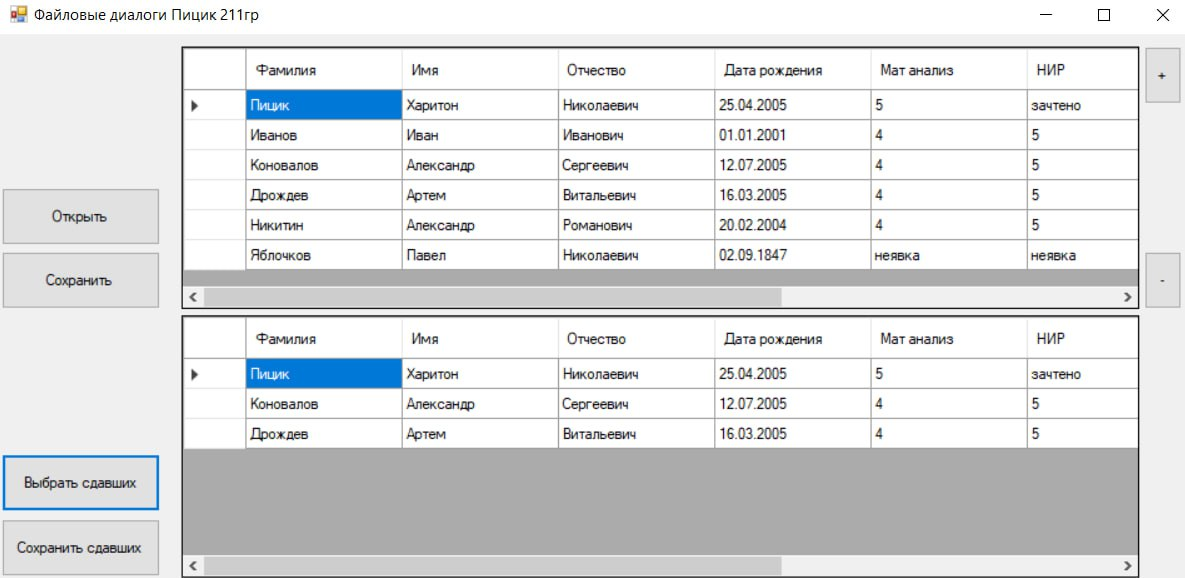
\includegraphics[scale=.45]{../img/files/files_choose.jpg}
\caption{<<Файловые диалоги>>: вид окна после выбора сдавших}
\label{fig:files_choose}
\end{figure}

При попытке добавить в исходную таблицу строку, содержащую некорректное значение даты или оценки, выводится ошибка 
(см. рисунок \ref{fig:files_error}).
\begin{figure}[H]
\centering
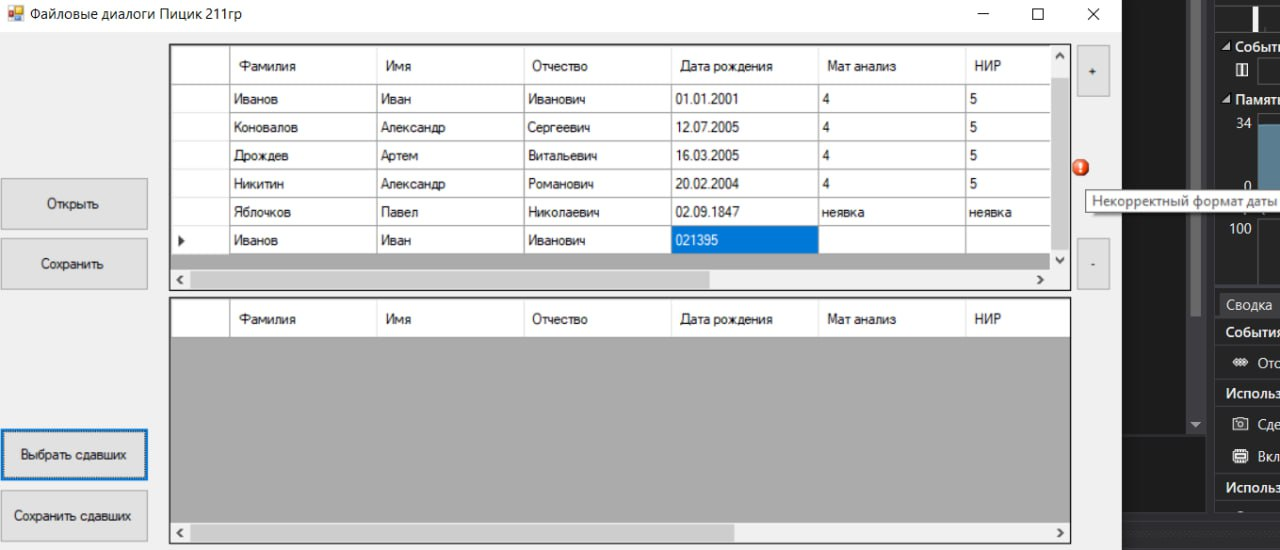
\includegraphics[scale=.45]{../img/files/files_error.jpg}
\caption{<<Файловые диалоги>>: вывод ошибки в окне программы}
\label{fig:files_error}
\end{figure}

Полный код программы приведён в приложении \ref{app:repo}.